\documentclass[a4paper,12pt]{article}

% UTF-8
\usepackage[utf8]{inputenc}
\usepackage{a4wide}

% Jinbo
\usepackage{hyperref}
\usepackage{graphicx}
\usepackage{float}
\usepackage{fancyhdr}

% BibTeX needs urls
\usepackage{booktabs}
\usepackage{hyperref}

\bibliographystyle{plain}

% Math - why not?
\usepackage{amsfonts}
\usepackage{amssymb}
\usepackage{amsmath}

% make the title page a bit smaller
\usepackage{titling}

% Force single spacing
\renewcommand{\baselinestretch}{1.0}

% Title Page
\newcommand*{\titleGM}{\begingroup % Create the command for including the title page in the document
	\thispagestyle{empty}
	\hbox{ % Horizontal box
		\hspace*{0.2\textwidth} % Whitespace to the left of the title page
		\rule{1pt}{\textheight} % Vertical line
		\hspace*{0.05\textwidth} % Whitespace between the vertical line and title page text
		\parbox[b]{0.75\textwidth}{ % Paragraph box which restricts text to less than the width of the page

			{\noindent\LARGE\bfseries Big Data Initiative: \\[0.5\baselineskip] Effective Caching in \\[0.5\baselineskip] Online Video Platforms}\\[2\baselineskip] % Title
			\\[4\baselineskip] % Tagline or further description
			{\large Rongrong Bao\ \ \ Atabak Hafeez\\[0.5\baselineskip] Tom Wiesing\ \ \ Jinbo Zhang} % Author name

			\vspace{0.45\textheight} % Whitespace between the title block and the publisher
		}}
		\endgroup}

\begin{document}

\titleGM

\clearpage
\vspace*{\fill}
\begin{abstract}
	Data on the internet grows by 50 percent annually. More than 90\% of the data has been generated in recent years. This is the time for big data. How can we effectively transfer this huge amount of data?

	We want to investigate caching techniques used by online video platforms and in particular by YouTube. YouTube is a leading online video provider worldwide. Before 2012, video streaming in YouTube was done using Real Time Messaging Protocol (RTMP)-based servers. This requires a streaming server and a near-continuous connection between the server and user. Requiring such a streaming server can increase implementation cost and RTMP-based video streaming is at risk of being blocked by firewalls. In 2012, this was replaced by HTTP (Hypertext Transfer Protocol) based servers known as MPEG DASH (Dynamic Adaptive Streaming over HTTP). HTTP is the protocol used by websites to bring their content to the users. By using this technology it was possible to use existing optimizations in the form of HTTP-Caching. This capability decreased total bandwidth costs associated with delivering the video since videos would be served from web-based caches rather than the origin server. This improved quality of service, since cached data is generally closer to the viewer and more easily retrievable.

	The essay will explain and discuss different kinds of caching techniques, optimizations, data analysis and prediction techniques used by YouTube, including their advantages/disadvantages and potential social impacts.
\end{abstract}
\vfill % equivalent to \vspace{\fill}
\clearpage

\newpage

\tableofcontents

\newpage
\section{Introduction}
What is Big Data? This question has become more and more important in recent years. A possible answer is given by Viktor Mayer-Schoenberg in \cite{Mayer-Schnberger:2013:BDR:2588165} where he refers to the fact that Big Data does not just use random analysis but uses all available data for analysis and processing. This answer does not completly answer the question. 

In this paper we focus on one of the major source of Big Data, the Internet. 
The United States Internet Data Center pointed out that the data on the Internet will soon grow by 50 percent annually. During a single day the internet today already generates new content to fit on 168 million DVDs. 2 million community posts are made every day. This is the same as number of letters that would be printed in 770 years of Time Magazine. The data produced by emails is much bigger. It fills 294 billion DVDs. As of 2012, the amount of data available on the Internet jumped from Terabyte (TB\footnote{1 TB is 1000 Gigabytes}) level via Petabyte (PB\footnote{1 PB is 1000 TB})) and Exabyte (EB\footnote{1 EB is 1000 TB}) level to the Zettabyte (ZB\footnote{1 ZB is 1000 EB}) level. The International Data Corporation (IDC) showed that by 2020 the size of worldwide generated data will reach 44 times the amount of today. 

As we have seen from the examples above Big Data Analysis is becoming more and more important. Real-time big data analytics can be of immense importance for a business. But a buisness must first evaluate pros and cons of this process as it is still a relatively new technology. It is expected to evolve in the future and hopefully resolve some of its current challenges. 

In this paper we will discuss YouTube -- the biggest video-sharing website in the world -- as a typical example of a video sharing platform that uses big data. We want to explaing what caching is, how it is used in YouTube and want to discuss its advantages and disadvantes. YouTube has an average of one hour of video uploads per second, and an average of 35 million video uploads daily. According to \cite{expandedramblings:stats}, YouTube now has more than 1 billion users, which is almost a third of total daily consumption of the world's Internet video viewing time. As of this year, YouTube's viewing time has increased by 60\%, which is on the highest level of growth. Without the process of development of Big Data, YouTube will not be able to keep up with the needs of the users in the world. 

In section \ref{whatiscaching} we will first introduce what caching is and give some basics on how YouTube makes use of this. Afterwards in section \ref{advantages} we will focus on this further and elaborate the advantages of YouTubes caching. After discussing the disadvantages of caching in section \ref{disadvantages} we finally conclude and reflect on the points we make in section \ref{conclusion}. 


\newpage
\section{What is Caching?}\label{whatiscaching}
Before we delve into the specifics of how Youtube does caching and the advantages and disadvantages of the different kinds of caching, we will explain how caching itself is and also explain the different possibilities available to use it in Youtube streaming.

Caching is a method to store data in cache. A cache is a basically temporary storage area on the local hard disk of a user. This storage area may contain data such HTML pages, images, files, and Web Projects in order to make it faster for the user to access it, which helps improve the efficiency of the computer and the overall efficiency of the task at hand. The important thing to note here is that occurs without the user knowing about it. For example, when a user returns to a Web page they have recently accessed, the browser can pull those files from the cache instead of the original server because it has stored the user?s activity. The storing of that information saves the user time by getting to it faster, and lessens the traffic on the network.


\subsection{Caching and Buffering in Youtube}
To explain caching in Youtube and how it has changed and updated, we also need to understand the notion of buffering. Buffering involves pre-loading data into a certain area of memory known as a "buffer". This is basically a a more specific kind of caching which Youtube uses to store the loaded video on to the local memory of the browser in use.

In 2013, Youtube made a design decision in their buffering system where they moved from Real Time Messaging Protocol (RTMP)-based Dynamic Streaming to MPEG DASH (Dynamic Adaptive Streaming over HTTP).

To a user, this is important because it changes the extent to which you can cache you Youtube video before viewing it. Basically, while Youtube was using RTMP-based Dynamic Streaming, if a user had a relatively slow connection, which would not allow them to view the video as smoothly as one would want, he could pause the video and view it later when the whole video is buffered or cached to the local storage of the browser. This technology required a near-continuous connection between the server - the original storage location where one's local computer is connected to retrieve the video - and the player on one's browser.

With Youtube's shift to using MPEG DASH, being able to buffer the whole video and then coming back to it was no longer possible. MPEG DASH use standard HTTP web servers to deliver streaming content, obviating the need for a streaming server. In addition, HTTP packets are firewall friendly and can utilise HTTP caching mechanisms on the web. To an average user, this means that now when he or she pauses a video because the video is not very smooth, the video buffers for a while and then stops buffering. The cache, hence, does not at this stage store the whole video. The only condition in which the video may cache the whole video is if you start the video and watch the whole way through. In this case, if the user turns off the internet, it would be possible for the user to re-watch the video without having to reload it from the server.

\subsection{Caching on the Servers}
So why did Youtube decide to make this significant change in their protocol? This is mainly because this makes streaming high quality videos more efficient because it can use caching on the servers.

Caching on the server means that when a user connects to a server, the connection is not direct. There is something in-between known as a caching server. The caching server acts as a web proxy server so it can serve those requests. After a web proxy server receives requests for web objects, it either serves the requests or forwards them to the origin server (the web server that contains the original copy of the requested information). Using MGEP DASH, Youtube was able to exploit this feature resulting in higher resolution videos being available to the user in a more efficient manner.

This form of caching also aims to make sure that the user can experience the best quality of video according to the available brandwidth speed. For example, a video may start playing at 360P resolution, but if the system detects that the brandwidth is now able to handle 720P, it will shift to that. Thus, using MPEG DASH, Youtube only caches chunks of the video and only a small chunk of them are loaded when a video is paused. 


\newpage
\section{Advantages of Caching}\label{advantages}
\ednote{Make subsections}
\ednote{A few intro words}
\ednote{what are DC and CDN solving?}

Notably, YouTube used two techniques to deliver web contents effectively -- Distributed Caching and Content Delivery Network.

A distributed cache is an extension of the traditional concept of cache used in a single locale. A distributed cache may span multiple servers so that it can grow in size and in transactional capacity\cite{wiki:dcache}. Before we talk about distributed caching technique more deeply, we will introduce some terms to help us better understand the idea behind it. In communication networks, a \textit{node} is either a connection point, a redistribution point, or a communication endpoint. Speaking of distributed network, the nodes are clients, servers or peers. By storing the data not on the individual web server's memory but on other cloud resources, \textit{distributed cache} offers high throughput, low-latency access to commonly accessed application data.

One significant advantage for distributed caching, is that when the application scales by adding or removing servers, or when servers are replaced due to upgrades or faults, the cached data remain accessible to every server that runs the application. For example, If we have data \texttt{1, 2, 3, 4, 5} and servers \texttt{A, B, C}, and we store \texttt{1, 2, 5} in \texttt{A}, \texttt{3, 5, 4} in B, \texttt{1, 2, 3, 4} in \texttt{C}. If one server is down, we won't lose any data, because every piece of data has a copy in another server.

\ednote{Graph needed here. Someone please?}

By distributing data efficiently and effectively, caching can dramatically improve application responsiveness. Comparing to access data from relational databases, which requires a lot computations, accessing data from cache is much faster. Caching works best for application workloads that do more reading than writing of data, and when application users share a lot of common data. So this is why such technique is very useful for YouTube: those popular videos will be watched again and again.

\begin{figure}[H]
	\centering
	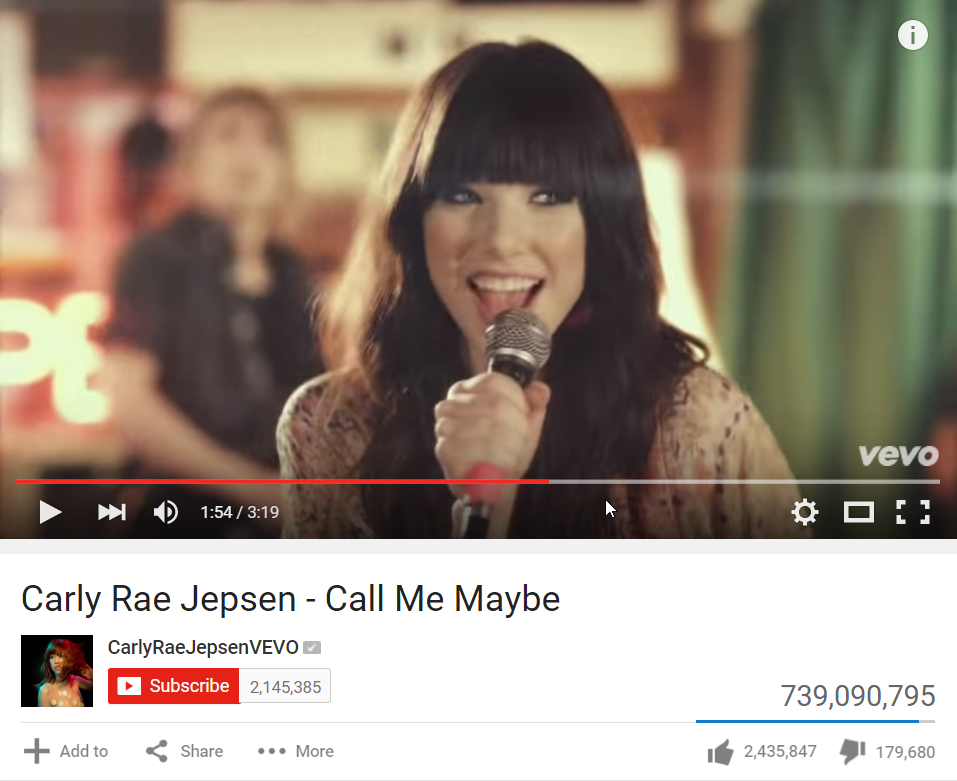
\includegraphics[width=0.7\linewidth]{CallMeMaybe.png}
	\caption{A very popular video in YouTube which is watched more than 700 million times}
\end{figure}

In order to get data from cache, the data must exist in cache before retrieving. There are several strategies for putting data into a cache \cite{azure:distributed}:
\begin{itemize}
	\item On Demand \ednote{try not to be so scary}

	The application tries to retrieve data from cache, and when the cache doesn't have the data (a "miss"), the application stores the data in the cache so that it will be available the next time. The next time the application tries to get the same data, it finds what it's looking for in the cache (a "hit").

	\item Background Data Push

	Background services push data into the cache on a regular schedule, and the application always pulls from the cache. This approach works great with high latency data sources that don't require you always return the latest data.
\end{itemize}

Strategy 2 is clearly the better for YouTube. YouTube will the count the watching times in order to filter the popular videos from non-popular ones, or count the watching times per minute in order to filter the trendy videos from the outdated ones, thus the background services have enough information to determine which videos will be pushed into cache. Also, once the video is uploaded, it will not change anymore, so the cached data will always stay tuned with the original one.

When we type \url{www.youtube.com} in our browser, how can they determine which server will respond our request? There are several different techniques for determining the responsive server, in this paper, we will mainly focus on one of the them -- \textit{Content Delivery Network}.

A \textit{Content Delivery Network} (or CDN for short) is a system of distributed network that delivers web pages and other web contents to a user based on the geographic locations of the user, the origin of the web page and a content delivery server \cite{webopedia:cdn}.

This service is effective in speeding the delivery of content of websites with high traffic and websites that have global reach. The closer the CDN server is to the user geographically, the faster the content will be delivered to the user. CDNs also provide protection from large surges in traffic.

Servers nearest to the website visitor respond to the request. The CDN copies the pages of a website to a network of servers that are dispersed at geographically different locations, caching the contents of the page. When a user requests a web page that is part of a content delivery network, the CDN will redirect the request from the originating site's server to a server in the CDN that is closest to the user and deliver the cached content. The CDN will also communicate with the originating server to deliver any content that has not been previously cached \ednote{These three part need to polish.}.

Thus, the CDN can reduce traffic on the primary network, which improves video content and web performance overall.


\newpage
\section{Disadvantages of Caching}\label{disadvantages}
While caching videos in the users web browser has many useful effects as discussed above it also has several bad side effects. In this section we will first explain some of the technical side effects and then continue discuss some social implications.

\subsection{Technical side effects}
In order to take advantage of caching of videos the browser needs to create caches for all the videos that the user plays. Additionally every time a video is played the browser has to check if a cached version of the video already exists. If this is the case the video can be played from the cached version. If this is not the case however the browser has to either create a cached version of the video or play a direct version from the server. Both of these decisions have a negative performance impact since the video has to be downloaded from the server which is slower then playing a local version.

Furthermore a cached version might not always be up-to-date. It is conceivable that when a news station has uploaded a video to YouTube and later on finds an error in their report that they might update their video in order to provide the most correct and up-to-date information. If this video has been cached by a viewer of the video they might no longer have the newest version available in their cache. Thus in order to use caches properly every time the cache is used the web browser needs to check if it is still up-to-date. This process can be further complicated if only parts of the video are cached. Furthermore if the cache is invalidated (meaning it is found to no longer be up-to-date) it is inefficient to reload the entire video if only parts of it have changed.

It is also possible that some videos are cached locally even though the user does not want to watch them. This is for example the case when advertisements are played before the video. They are not desired by the user and might nonetheless be cached. Sometimes the users might also watch a few seconds of the beginning of the video and then decide not to watch the remaining part. This can cause both a waste of bandwidths and local hard drive spaces.

Since caching technically copies the videos from the server to the hard disks of the local user, the video is no longer stored in only one central location. That means that even if the video has to be deleted, for example for legal reasons, it might still be available locally. This might result in legal hurdles if a license has to be obtained in order to show the video.

Additionally some of the videos the user watches might remain cached on the users hard drive even after they have watched the video. While a single video does not take too much space this can cause a problem if there are many of these cached videos. It is especially important for mobile users as these typically have less space available on their devices. Furthermore the user might not want a record of the videos they watched for privacy reasons.

\subsection{Social implications}
When using predictive caching YouTube (or other online video providers) are using data from the user. They try to analyse the videos the user has watched in the past and want to predict which videos the user might watch in the future. Some users might not desire getting videos predicted for several reasons. Especially when on a connection with limited bandwidth the user might object to having this bandwidth used up with videos that he might not watch anyways.

Additionally several users might not want their video history to be recorded. This can easily be considered an intrusion into the users privacy. This information could also be used against the user especially when the wrong videos are predicted by the algorithm.

YouTube sells anonymized customer data to advertisers. If sold to advertisers, this data is commonly used to predict products the user might be interested in. Related adverts are then played on the next video the user watches. This brings money to the content provider but does not give any significant advantage to the user.


\newpage
\section{Conclusion}\label{conclusion}
In this paper we have talked about caching techniques, how they are used by YouTube in particular, and they relate to Big Data. This is an era of data explosion, if we don't have such a substantial size of data, caching techniques won't be so essential to those online video platforms. We have discussed how caching enables the watching of videos on the Internet by downloading the video onto the hard disk of the local computer. We have mentioned how techniques like distributed caching or the concept of CDNs can increase user experiences from the technical side. Even though this brings a lot of advantages we have also seen how this can have negative side effects and other social implications.

These side effects are still open for discussing, Clearly there's no elixir for the problems, and they  cannot be solved by technical solutions alone. Social impacts need to be considered and, like almost every other use of Big Data, this involves taking privacy issues into account. In general (Big) Data collection always has good and bad effects. The disadvantages mostly come from privacy issues whereas the advantages primarily come from the fact that it can make technical solutions more efficient. 

It makes sense to let users decide, to offer options to the them. A controversial issue related to each individual should be solved by themselves -- after all, people are different from each other. They can decide if they want a better experience in their services or a better protection of their privacy.  

It also makes sense to improve the transparency of data usage. Probably everyone enjoys better experience, but some of them are more concerned about if they are monitored by someone or some institution. For the data collectors, if they can offer more concrete evidences, to show that the collected data are encrypted, are stored safely, and they won't be decrypted by any malicious people, or be transferred as other usages, then these movements can certainly reassure some worried people.




\newpage
\renewcommand\refname{\vskip -1cm}
\section{Bibliography}

\nocite{hwu:procon}
\nocite{MPEGDASH}
\nocite{citrix:caching}
\nocite{OnlineVideoBandwagon}
\nocite{ats:caching}
\nocite{expandedramblings:stats}
\nocite{techopedia:weighing}

\bibliography{draft}
\end{document}
